%%%%%%%%%%%%%%%%%%%%%%%%%%%%%%%%%%%%%%%%%%%%%%%%%%%%%%%%%%%%%%%
%% OXFORD THESIS TEMPLATE

% Use this template to produce a standard thesis that meets the Oxford University requirements for DPhil submission
%
% Originally by Keith A. Gillow (gillow@maths.ox.ac.uk), 1997
% Modified by Sam Evans (sam@samuelevansresearch.org), 2007
% Modified by John McManigle (john@oxfordechoes.com), 2015
% Modified by Ulrik Lyngs (ulrik.lyngs@cs.ox.ac.uk), 2018, for use with R Markdown
%
% Ulrik Lyngs, 25 Nov 2018: Following John McManigle, broad permissions are granted to use, modify, and distribute this software
% as specified in the MIT License included in this distribution's LICENSE file.
%
% John tried to comment this file extensively, so read through it to see how to use the various options.  Remember
% that in LaTeX, any line starting with a % is NOT executed.  Several places below, you have a choice of which line to use
% out of multiple options (eg draft vs final, for PDF vs for binding, etc.)  When you pick one, add a % to the beginning of
% the lines you don't want.


%%%%% CHOOSE PAGE LAYOUT
% The most common choices should be below.  You can also do other things, like replacing "a4paper" with "letterpaper", etc.

% This one will format for two-sided binding (ie left and right pages have mirror margins; blank pages inserted where needed):
%\documentclass[a4paper,twoside]{templates/ociamthesis}
% This one will format for one-sided binding (ie left margin > right margin; no extra blank pages):
%\documentclass[a4paper]{ociamthesis}
% This one will format for PDF output (ie equal margins, no extra blank pages):
%\documentclass[a4paper,nobind]{templates/ociamthesis}
%UL 2 Dec 2018: pass this in from YAML
\documentclass[a4paper, nobind]{templates/ociamthesis}


% UL 30 Nov 2018 pandoc puts lists in 'tightlist' command when no space between bullet points in Rmd file
\providecommand{\tightlist}{%
  \setlength{\itemsep}{0pt}\setlength{\parskip}{0pt}}
 
% UL 1 Dec 2018, fix to include code in shaded environments

%UL 2 Dec 2018 reduce whitespace around verbatim environments
\usepackage{etoolbox}
\makeatletter
\preto{\@verbatim}{\topsep=0pt \partopsep=0pt }
\makeatother

%UL 26 Mar 2019, enable strikethrough
\usepackage[normalem]{ulem}

%UL 15 Oct 2019, enable link highlighting to be turned off from YAML
\usepackage[colorlinks=false,pdfpagelabels,hidelinks=true]{hyperref}

%%%%% SELECT YOUR DRAFT OPTIONS
% Three options going on here; use in any combination.  But remember to turn the first two off before
% generating a PDF to send to the printer!

% This adds a "DRAFT" footer to every normal page.  (The first page of each chapter is not a "normal" page.)

% This highlights (in blue) corrections marked with (for words) \mccorrect{blah} or (for whole
% paragraphs) \begin{mccorrection} . . . \end{mccorrection}.  This can be useful for sending a PDF of
% your corrected thesis to your examiners for review.  Turn it off, and the blue disappears.
\correctionstrue

%%%%% BIBLIOGRAPHY SETUP
% Note that your bibliography will require some tweaking depending on your department, preferred format, etc.
% The options included below are just very basic "sciencey" and "humanitiesey" options to get started.
% If you've not used LaTeX before, I recommend reading a little about biblatex/biber and getting started with it.
% If you're already a LaTeX pro and are used to natbib or something, modify as necessary.
% Either way, you'll have to choose and configure an appropriate bibliography format...

% The science-type option: numerical in-text citation with references in order of appearance.
% \usepackage[style=numeric-comp, sorting=none, backend=biber, doi=false, isbn=false]{biblatex}
% \newcommand*{\bibtitle}{References}

% The humanities-type option: author-year in-text citation with an alphabetical works cited.
% \usepackage[style=authoryear, sorting=nyt, backend=biber, maxcitenames=2, useprefix, doi=false, isbn=false]{biblatex}
% \newcommand*{\bibtitle}{Works Cited}

%UL 3 Dec 2018: set this from YAML in index.Rmd
\usepackage[style=authoryear, sorting=nyt, backend=biber, maxcitenames=2, useprefix, doi=true, isbn=false, uniquename=false]{biblatex}
\newcommand*{\bibtitle}{Works Cited}

% This makes the bibliography left-aligned (not 'justified') and slightly smaller font.
\renewcommand*{\bibfont}{\raggedright\small}

% Change this to the name of your .bib file (usually exported from a citation manager like Zotero or EndNote).
\addbibresource{references.bib}


% Uncomment this if you want equation numbers per section (2.3.12), instead of per chapter (2.18):
%\numberwithin{equation}{subsection}


%%%%% THESIS / TITLE PAGE INFORMATION
% Everybody needs to complete the following:
\title{Analyzing the Feature Importance of Different Variables on the Price of Ikea Products}
\author{Philip Krück, Johannes Pein}
\college{}

% Master's candidates who require the alternate title page (with candidate number and word count)
% must also un-comment and complete the following three lines:
%\masterssubmissiontrue
%\candidateno{933516}
%\wordcount{28,815}

% Uncomment the following line if your degree also includes exams (eg most masters):
%\renewcommand{\submittedtext}{Submitted in partial completion of the}
% Your full degree name.  (But remember that DPhils aren't "in" anything.  They're just DPhils.)
\degree{B.Sc. Business Informatics (18A-BI)}
% Term and year of submission, or date if your board requires (eg most masters)
\degreedate{04.12.2020}


%%%%% YOUR OWN PERSONAL MACROS
% This is a good place to dump your own LaTeX macros as they come up.
\modulename{Digital Toolbox: Data Business}
\lecturer{Lecturer: Ulf Köther}
\groupnumber{Group Number: 7}
\matriculationnumbers{Matriculation Numbers: 3938 (P.Krück), 4001 (J.Pein)}


% To make text superscripts shortcuts
	\renewcommand{\th}{\textsuperscript{th}} % ex: I won 4\th place
	\newcommand{\nd}{\textsuperscript{nd}}
	\renewcommand{\st}{\textsuperscript{st}}
	\newcommand{\rd}{\textsuperscript{rd}}

%%%%% THE ACTUAL DOCUMENT STARTS HERE
\begin{document}

%%%%% CHOOSE YOUR LINE SPACING HERE
% This is the official option.  Use it for your submission copy and library copy:
\setlength{\textbaselineskip}{22pt plus2pt}
% This is closer spacing (about 1.5-spaced) that you might prefer for your personal copies:
%\setlength{\textbaselineskip}{18pt plus2pt minus1pt}

% You can set the spacing here for the roman-numbered pages (acknowledgements, table of contents, etc.)
\setlength{\frontmatterbaselineskip}{17pt plus1pt minus1pt}


% UL: You can set the general paragraph spacing here - I've set it to 2pt (was 0) so
% it's less claustrophobic
\setlength{\parskip}{2pt plus 1pt}


% Leave this line alone; it gets things started for the real document.
\setlength{\baselineskip}{\textbaselineskip}


%%%%% CHOOSE YOUR SECTION NUMBERING DEPTH HERE
% You have two choices.  First, how far down are sections numbered?  (Below that, they're named but
% don't get numbers.)  Second, what level of section appears in the table of contents?  These don't have
% to match: you can have numbered sections that don't show up in the ToC, or unnumbered sections that
% do.  Throughout, 0 = chapter; 1 = section; 2 = subsection; 3 = subsubsection, 4 = paragraph...

% The level that gets a number:
\setcounter{secnumdepth}{2}
% The level that shows up in the ToC:
\setcounter{tocdepth}{2}


% JEM: Pages are roman numbered from here, though page numbers are invisible until ToC.  This is in
% keeping with most typesetting conventions.
\begin{romanpages}

% Title page is created here
\maketitle

%%%%% MINI TABLES
% This lays the groundwork for per-chapter, mini tables of contents.  Comment the following line
% (and remove \minitoc from the chapter files) if you don't want this.  Un-comment either of the
% next two lines if you want a per-chapter list of figures or tables.
  \dominitoc % include a mini table of contents

% This aligns the bottom of the text of each page.  It generally makes things look better.
\flushbottom

% This is where the whole-document ToC appears:
\tableofcontents

%%%%% LIST OF ABBREVIATIONS
% This example includes a list of abbreviations.  Look at text/abbreviations.tex to see how that file is
% formatted.  The template can handle any kind of list though, so this might be a good place for a
% glossary, etc.
% First parameter can be changed eg to "Glossary" or something.
% Second parameter is the max length of bold terms.
\begin{mclistof}{List of Abbreviations}{3.2cm}

\item[R] Statistical Programming Language
\item[MSE] Mean Squared Error
\item[IQR] Interquartile Range

\end{mclistof} 


% The Roman pages, like the Roman Empire, must come to its inevitable close.
\end{romanpages}

%%%%% CHAPTERS
% Add or remove any chapters you'd like here, by file name (excluding '.tex'):
\flushbottom

% all your chapters and appendices will appear here
\hypertarget{intro}{%
\chapter{Introduction}\label{intro}}

This project report is an examination at the Hamburg School of Business Administration in the module `Data Business' as a part of a Bachelor of Science degree program. The students were given a data set and the task was to first explore the data and then choose a research question which was to be answered scientifically with the help of the statistical programming language R. The authors of this report were given a data set which contains Ikea products and different features, such as price, dimensional measures, name, category and designers of the product.

\hypertarget{theoretical-background-research-question}{%
\chapter{Theoretical Background \& Research Question}\label{theoretical-background-research-question}}

\hypertarget{data-set}{%
\section{Data Set}\label{data-set}}

\textcolor{gray}{by P. Krück}
The data set was obtained by a kaggle.com user (Reem Abdulrahman) by the means of webscraping techniques from the Saudi Arabian Ikea website in the furniture category on the 20th of April 2020. Noteworthy features include the name, category, price in Saudi Riyals, the designer and dimensions (width, height and depth). The data set has 13 variables and 2962 distinct observations after removing duplicates.

\hypertarget{theoretical_background}{%
\section{Theoretical Background}\label{theoretical_background}}

\hypertarget{random-forest-basics}{%
\subsection{Random Forest Basics}\label{random-forest-basics}}

\textcolor{gray}{by J. Pein}

In order to analyze the feature importance in relation to the price variable, a random forest regression model was chosen. A random forest consists of many decision trees, which make a prediction based on a majority decision process. In standard decision trees, each nodes is split to achieve the best performing model. In random forests however, the nodes are randomly split. Compared to linear regression models, the random forests model not only takes into account the mean and covariance structure of response, but also deeper deeper aspects of data\footnote{Grömping, ``Variable Importance Assessment in Regression: Linear Regression versus Random Forest.''} resulting in a more advanced and robust model.

\hypertarget{feature-importance}{%
\subsection{Feature Importance}\label{feature-importance}}

\textcolor{gray}{by J. Pein}

\begin{itemize}
\tightlist
\item
  feature and predictor variable can be used interchangibly
\end{itemize}

\hypertarget{research_question}{%
\section{Research Question}\label{research_question}}

\textcolor{gray}{by P. Krück}
This paper explores the influence for different variables on the price in the given data set. The motivating forces for this research question are the possible implications for price determination of new items.

\hypertarget{methods}{%
\chapter{Methods}\label{methods}}

\hypertarget{datacleaning}{%
\section{Data Cleaning and Transformatoin}\label{datacleaning}}

\textcolor{gray}{by P. Krück}
To examine the given data set properly, the authors first had to restructure and reformat it. This initial data cleaning step included type conversion, value mutation, addition of newly calculated fields and the removal of irrelevant columns.
Concretely, name, category and designer were converted to categorical variables. In the designer column, blank strings and values prefixed by ``IKEA of Sweden'' were converted to missing values (\texttt{NA}). Furthermore, both the price and old price were converted to double values and the currency was changed from Saudi Arabian Riyals to Euros based on the exchange rate from the time the data set was obtained by the author @ref(\#theoretical\_background).

Interestingly, the data set had a peculiarity where some rows were exact duplicates except for the category value. The authors considered multiple approaches to handle these data duplications without losing information about the category of an item.

One considered option was to merge the two category values into one column value via comma separation (e.g. \texttt{"a"} and \texttt{"b"} converts to \texttt{"a,\ b"}). However, this approach leads to the creation of many combinatorial categories with a low count of items per category which also reduces the item count per category where the category isn't comma separated. Overall this would lead to having many small categories which increases the difficulty in applying a regression model due to overfitting @ref(\#overfitting).

The second option was to create separate columns for the different values of \texttt{category}. The data set would then have observations with category one, two and three. While no information is lost utilizing this approach, most observations in the second and third category column would contain missing values, thus increasing the difficulty of analysis using a predefined model @\ref(\#random\_forest\_model).

The authors chose the option of selecting the observations out of the duplicates where the category count occurred most frequently when considering duplicates. The most important categories could be retained without including more column vectors into the data set as in option two.

To better facilitate the comparison of the different sizes of furniture items, the size in cubic meters was computed based on the depth, width and height values, and added as a column vector for further analysis.
Finally, the authors only selected columns that could have a potential impact on the analysis @ref(\#research\_question) for further investigation. A detailed comparison of the initial vs.~transformed data structure can be seen in tables \ref{tab:initial-ikea} and \ref{tab:tidy-ikea}.

TODO: Format these tables

\begin{table}

\caption{\label{tab:initial-ikea}Initial Data Set formatting.}
\centering
\begin{tabular}[t]{r|r|l|l|r|l|l|l|l|l|l|r|r|r}
\hline
X1 & item\_id & name & category & price & old\_price & sellable\_online & link & other\_colors & short\_description & designer & depth & height & width\\
\hline
0 & 90420332 & FREKVENS & Bar furniture & 2650 & No old price & TRUE & https://www.ikea.com/sa/en/p/frekvens-bar-table-in-outdoor-black-90420332/ & No & Bar table, in/outdoor,          51x51 cm & Nicholai Wiig Hansen & NA & 99 & 51\\
\hline
1 & 368814 & NORDVIKEN & Bar furniture & 9950 & No old price & FALSE & https://www.ikea.com/sa/en/p/nordviken-bar-table-black-00368814/ & No & Bar table,          140x80 cm & Francis Cayouette & NA & 105 & 80\\
\hline
2 & 9333523 & NORDVIKEN / NORDVIKEN & Bar furniture & 20950 & No old price & FALSE & https://www.ikea.com/sa/en/p/nordviken-nordviken-bar-table-and-4-bar-stools-black-black-s09333523/ & No & Bar table and 4 bar stools & Francis Cayouette & NA & NA & NA\\
\hline
3 & 80155205 & STIG & Bar furniture & 690 & No old price & TRUE & https://www.ikea.com/sa/en/p/stig-bar-stool-with-backrest-black-silver-colour-80155205/ & Yes & Bar stool with backrest,          74 cm & Henrik Preutz & 50 & 100 & 60\\
\hline
4 & 30180504 & NORBERG & Bar furniture & 2250 & No old price & TRUE & https://www.ikea.com/sa/en/p/norberg-wall-mounted-drop-leaf-table-white-30180504/ & No & Wall-mounted drop-leaf table,          74x60 cm & Marcus Arvonen & 60 & 43 & 74\\
\hline
5 & 10122647 & INGOLF & Bar furniture & 3450 & No old price & TRUE & https://www.ikea.com/sa/en/p/ingolf-bar-stool-with-backrest-white-10122647/ & No & Bar stool with backrest,          63 cm & Carina Bengs & 45 & 91 & 40\\
\hline
\end{tabular}
\end{table}

\begin{table}

\caption{\label{tab:tidy-ikea}Data Set after cleaning process.}
\centering
\begin{tabular}[t]{l|l|r|r|l|l|l|r}
\hline
name & category & price\_eur & old\_price\_eur & sellable\_online & other\_colors & designer & size\_m3\\
\hline
FREKVENS & Bar furniture & 65.02 & NA & TRUE & FALSE & Nicholai Wiig Hansen & NA\\
\hline
NORDVIKEN & Bar furniture & 244.14 & NA & FALSE & FALSE & Francis Cayouette & NA\\
\hline
NORDVIKEN / NORDVIKEN & Bar furniture & 514.05 & NA & FALSE & FALSE & Francis Cayouette & NA\\
\hline
STIG & Bar furniture & 16.93 & NA & TRUE & TRUE & Henrik Preutz & 0.30\\
\hline
NORBERG & Bar furniture & 55.21 & NA & TRUE & FALSE & Marcus Arvonen & 0.19\\
\hline
INGOLF & Bar furniture & 84.65 & NA & TRUE & FALSE & Carina Bengs & 0.16\\
\hline
\end{tabular}
\end{table}

\hypertarget{tbd}{%
\section{Exploratory Data Analysis}\label{tbd}}

\textcolor{gray}{by P. Krück}
The following sections explore our data based on the eight step data exploration protocol proposed by Zuur et al.\footnote{Zuur, ``A protocol for data exploration to avoid common statistical problems.''}

\hypertarget{step-1-outliers-in-price-and-independent-variables}{%
\subsection{Step 1: Outliers in Price and Independent Variables}\label{step-1-outliers-in-price-and-independent-variables}}

\textcolor{gray}{by P. Krück}
Outliers of the chosen variables (from tidying see @ref(\#datacleaning) can be observed for each variable (see plot \ldots{}).
The authors assume that outliers do not occur randomly in the form of an observer error. Web scraping code is written in a generic form which makes it generalizable to all applied pages. Thus takes human observation errors out of the equation. Additionally, the authors looked at individual outlier (stichprobenartig) examples and used the provided link column to manually double check observations against machine errors.
By the stated assumption, all outliers are meaningful for further analysis.

\hypertarget{step-2-homogeneity-of-price}{%
\subsection{Step 2: Homogeneity of Price}\label{step-2-homogeneity-of-price}}

\textcolor{gray}{by P. Krück}
The homogeneity (homoscedasticity) of variance for price is explored by the means of conditional boxplotting.
Within each name, and within each category the variance is heterogenous (see fig. \ref{fig:homogeneity}). However, looking at both name and category in conjunction, it is possible to explore homoscedasticity of variance for price.

In the context of this paper, the authors weren't able to inspect all variable combinations for the five categorical variables (\(2^3=8\)).

\begin{figure}
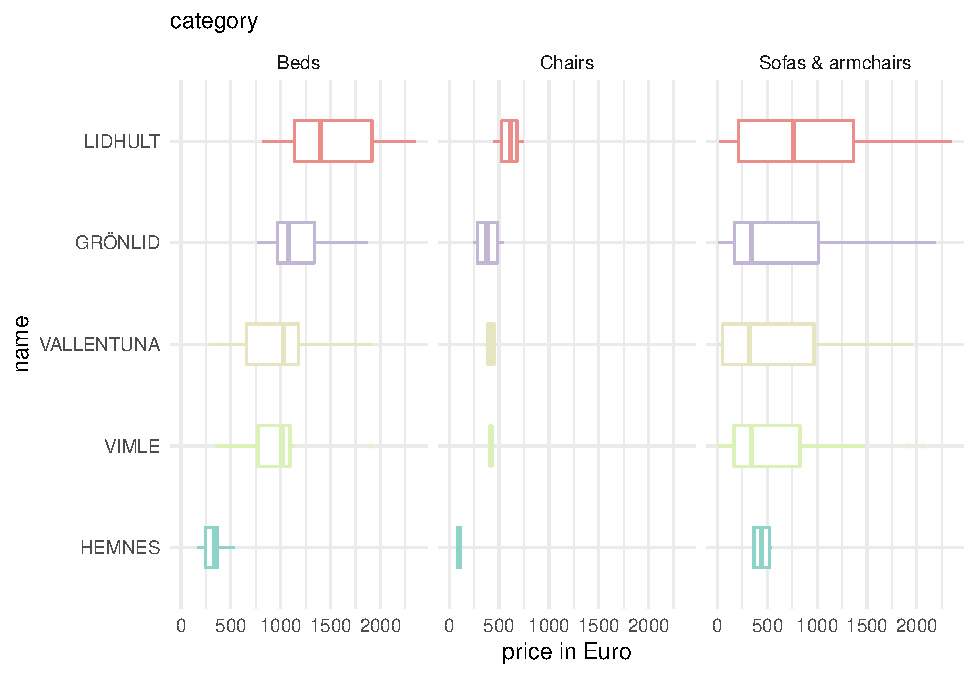
\includegraphics[width=1\linewidth]{_main_files/figure-latex/homogeneity-1} \caption{Homogeneity of category for selected combinations of name and category}\label{fig:homogeneity}
\end{figure}

\hypertarget{step-3-normality}{%
\subsection{Step 3: Normality}\label{step-3-normality}}

\textcolor{gray}{by P. Krück}
All numerical variables (\texttt{price}, \texttt{old\_price} and \texttt{size\_m3}) aren't arranged along a normal distribution (see fig. \ref{fig:normality}), but rather follow an exponential decay (\(e^{-x}\)).

\begin{figure}
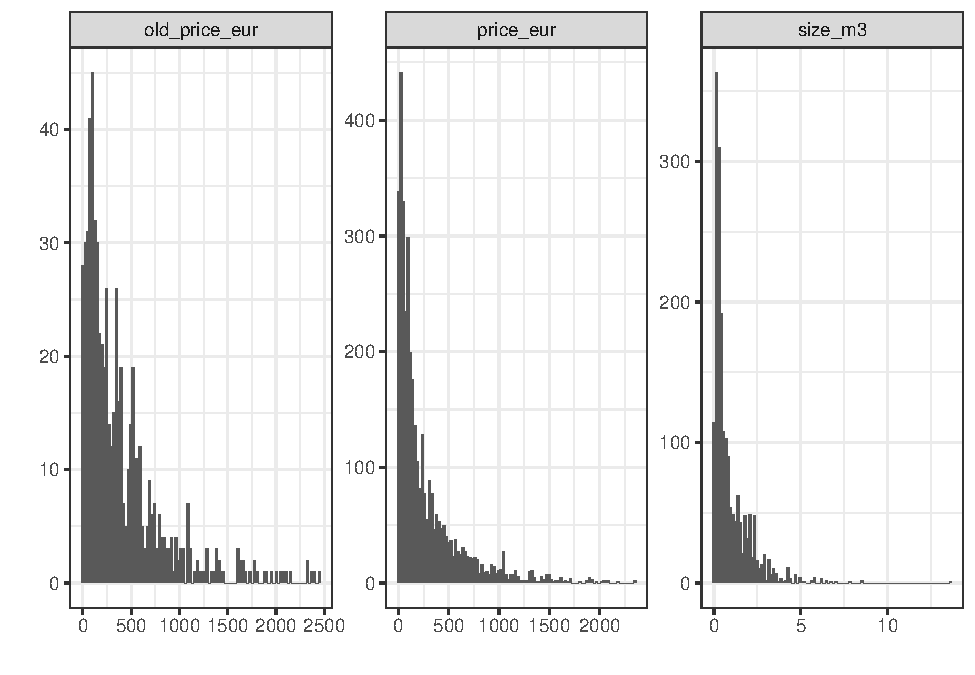
\includegraphics[width=1\linewidth]{_main_files/figure-latex/normality-1} \caption{Homogeneity of category for selected combinations of name and category}\label{fig:normality}
\end{figure}

\hypertarget{step-4-missing-values}{%
\subsection{Step 4: Missing Values}\label{step-4-missing-values}}

\textcolor{gray}{by P. Krück}
All variables were examined for missing values. Only \texttt{designer}, \texttt{size\_m3} and \texttt{old\_price\_eur} have missing values of 3.44\%, 45.9\% and 81\% respectively (see fig. \ref{fig:missing-values})).
The missing values for designer were deliberately set to \texttt{NA} by the authors in the case where the values contained digits, which is clearly a scraping error.
The \texttt{NA} values for the size can be explained due to the computation of this column vector. \texttt{size\_m3} is the product of \texttt{depth}, \texttt{width} and \texttt{height}. If one of those three values is missing, the end result is also a missing value.
The abscence of the old price variables is due to the fact that most items aren't on sale and thus don't have a missing value.

\begin{figure}
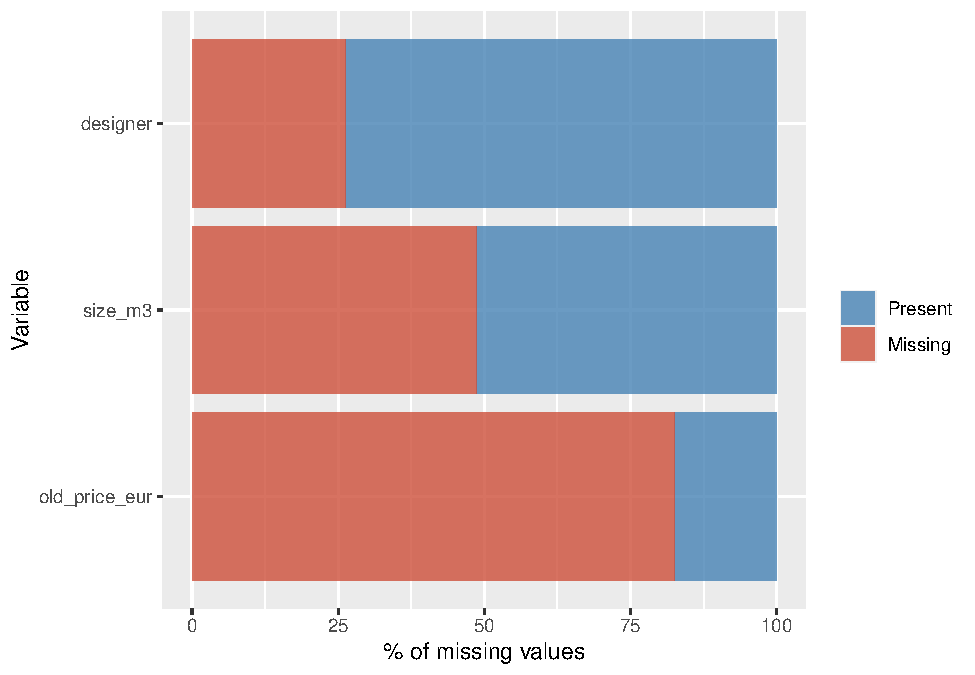
\includegraphics[width=1\linewidth]{_main_files/figure-latex/missing-values-1} \caption{Homogeneity of category for selected combinations of name and category}\label{fig:missing-values}
\end{figure}

\hypertarget{step-5-collinearity-between-independent-variables}{%
\subsection{Step 5: Collinearity between Independent Variables}\label{step-5-collinearity-between-independent-variables}}

\textcolor{gray}{by P. Krück}
The old price has a rather high VIF which corresponds to high multicollinearity (see table \ldots{}). Contrarily, size has a low VIF which translates to low multicollinearity among the other independent variables (see table \ldots{}).

TODO: use values from step 5 of eda protocol

\begin{table}

\caption{\label{tab:initial-ikea2}Initial Data Set formatting.}
\centering
\begin{tabular}[t]{r}
\hline
x\\
\hline
1\\
\hline
3\\
\hline
4\\
\hline
\end{tabular}
\end{table}

\hypertarget{relationship}{%
\subsection{Step 6: Relationship between Independent Variables and Price}\label{relationship}}

Inspecting the relationship between the independent variables and price strong relationships between \texttt{old\_price\_eur} and \texttt{size\_m3} can be observed, while no relationship can be observed for the other variables (see \ref{fig:relationship-x-y}).
\texttt{old\_price\_eur} has a linear relationship (see fig. \ref{fig:relationship-old-price}) whereas \texttt{size\_m3} fits a second order polynomial (see fig. \ref{fig:relationship-size-m3}) to price.

\begin{figure}
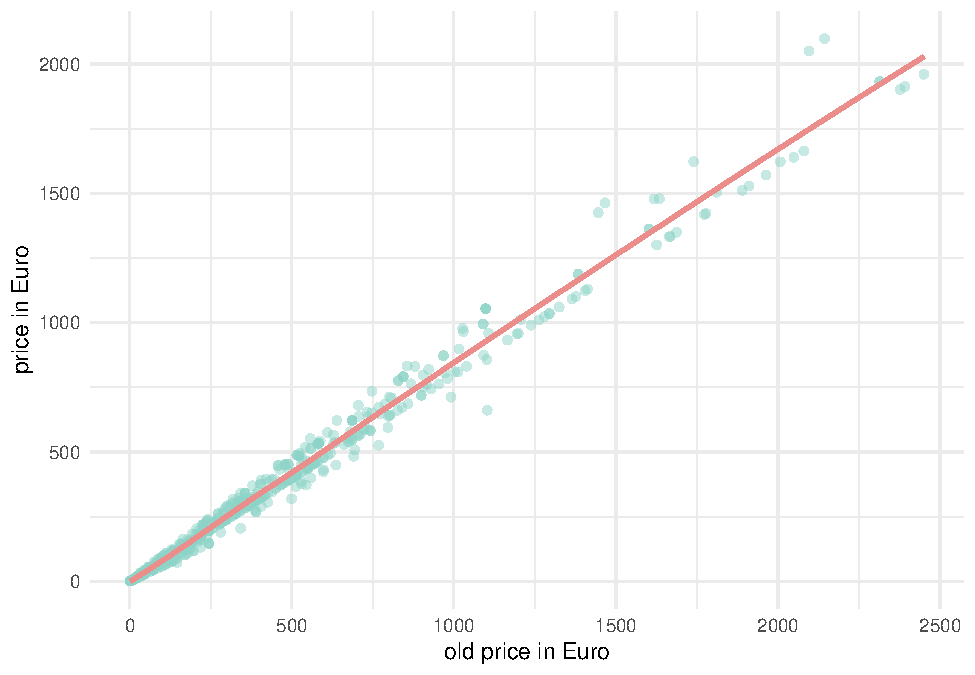
\includegraphics[width=1\linewidth]{_main_files/figure-latex/relationship-old-price-1} \caption{caption}\label{fig:relationship-old-price}
\end{figure}

\begin{figure}
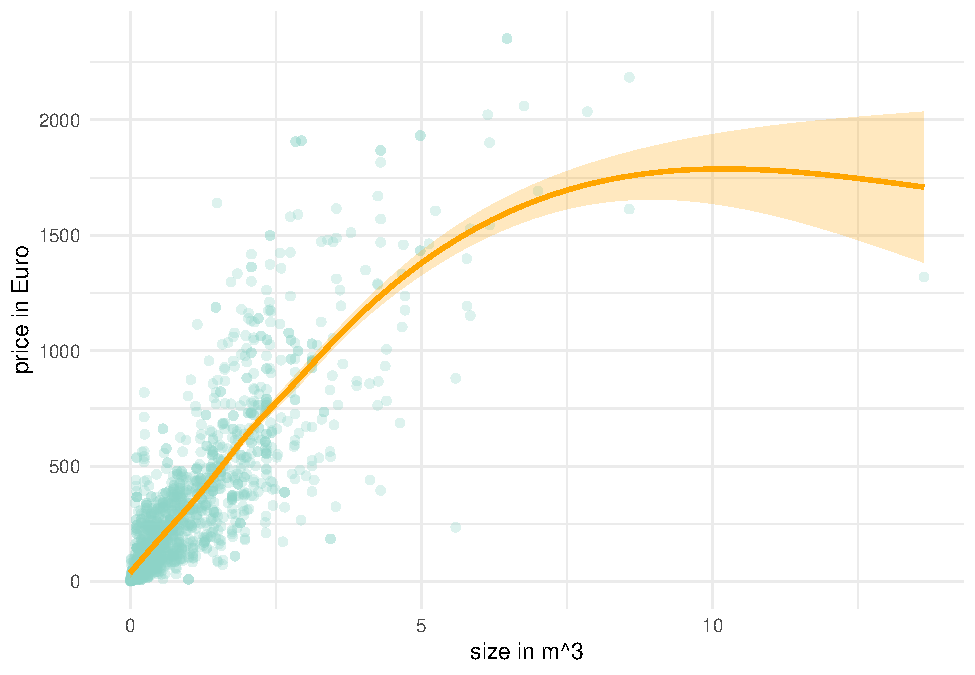
\includegraphics[width=1\linewidth]{_main_files/figure-latex/relationship-size-m3-1} \caption{caption}\label{fig:relationship-size-m3}
\end{figure}

\hypertarget{step-7-interactions}{%
\subsection{Step 7: Interactions}\label{step-7-interactions}}

The interactions between different variables is explored by the means of coplotting.
Using this form plotting the relationship of two numerical variables is explored by creating a matrix of plots subdivided by two categorical variables.
In the given data set there are three numerical and three categorical variables which can be explored in this form of interaction. For the numerical variables, \texttt{old\_price\_eur} has such a strong relationship with price (see \ldots{}) that a more detailed breakdown by the categorical variables wouldn't reveal new information. This leaves the exploration of \texttt{size\_m3} and \texttt{price\_eur} broken down by designer, name and category resulting in (3 out of 2 = 3) combinations of coplots.
Unfortunately, the authors of this papers weren't able to fully explore all combinations due to programming difficulties.
Plotting designer and name works \ldots{}.

\begin{itemize}
\item
  Coplotting designer and name works, while the two combination would not plot
\item
  The linear model predicted infinite values and thus coplot the values properly for the other two options
\item
  However, dropping all NA values and thus reducing the total data size to 354 observations would case for the combination coplot name and category while name + designer combination would not work
\item
  The authors hypothesized that infinite values were caused by a division of zeros of the linear model since there occured 0 values in size
\item
  This however proved to be wrong after applying respective filters
\item
  The following interaction could be analyzed
\item
  \begin{itemize}
  \tightlist
  \item
    There is probably no significant interaction between size, price, name \& designer as can be seen in coplot -\textgreater{} lines are nearly parallel
  \end{itemize}
\item
  Based on the coplot of category and name with the 354 observations, inparallelity could be observed and thus could conclude a interaction. However, this could also be due to the small sample size
\item
\end{itemize}

(footnote): the authors would highly appreciate any solutions on this matter\footnote{This is a footnote.}

\hypertarget{step-8-independence-of-price}{%
\subsection{Step 8: Independence of Price}\label{step-8-independence-of-price}}

\begin{itemize}
\tightlist
\item
  Durch das tidying in (cross reference) duplicate removal -\textgreater{} Zuur paper Step 8 1. citation: meaning that information from any one observation should not provide information on another after the effects of other variables have been accounted for. This concept is best explained with examples.
\end{itemize}

\hypertarget{rf}{%
\section{Random Forest Regression Model}\label{rf}}

\textcolor{gray}{by J. Pein}

TODO: Students should decide on an appropriate statistical procedure to answer their chosen research questionand should state any prerequisites /assumptions of this methodaccordingly.

This analysis was conducted using the R randomForest package, which is based on the original Breiman and Cutler's Fortran code for random forest regression. To learn more about how random forests work or the randomForest package, see Liaw and Wiener\footnote{``Classification and Regression by randomForest.''} or \#chapter2 \#TODO. To reproduce the analysis conducted in this paper, the prepatory steps are described here. The following steps are based on an already cleaned ikea data frame which is described in \ref{datacleaning}. This data frame is then transformed further to be used with the randomForest package.

First, the variable \texttt{old\_price\_eur} is removed from the data frame, due to a very high correlation and relationship to the price variable analyzed in \ref{collinearity} and \ref{relationship} Then, the designers and names, which are not part of the 50 \texttt{designers} and 49 \texttt{names} with the highest number of occurences, are grouped in the \texttt{other} value. This is because the \texttt{randomForest} method does not allow categorical variables with more than 53 predictors. The last step is dealing with the missing values in the data. As described in \ref{zeros}, there are missing values in the \texttt{size\_m3} and \texttt{designer} variables. To use the \texttt{randomForest} method of the randomForest package on the data, those missing values are dealt with using three different approaches. In the first approach the rows with missing values are deleted, reducing the total number of rows by aproximately 50\%. In the second approach the missing values are dummy coded with a value of -1000. The third approach uses the \texttt{na.roughfix\ =\ na.omit} argument, which is the built in way of the randomForest package to deal with missing values.
After preparing the data, the \texttt{randomForest} method of the randomForest package is applied to the data with number of trees set to 2000 and importance set to \texttt{TRUE}.

\texttt{randomForest(price\_eur\ \textasciitilde{}\ .,\ rf\_ikea,\ ntree=2000,\ keep.forest=FALSE,\ importance=TRUE)}

Then the \texttt{importance} method of the randomForest package is used to save the feature importances, which are computed by permuting feature importance, which is described in \#chapter2 \#TODO. The three different approaches of dealing with the missing values in the data set lead to different results, so the authors chose to calculate the mean result of the three approaches. The result of this analysis is presented in the following chapter.

\hypertarget{results}{%
\chapter{Results}\label{results}}

\hfill\textcolor{gray}{by J. Pein}

TODO: set n\_trees to 2000 before handing in
TODO: The results sectionshould comprise all necessary calculations, including checking of assumptions (if applicable), which are thendiscussedinconnection with the research questionin the following section.

In this chapter, the results of the analysis of the feature importance of different predictor variables (features) on the response variable price of Ikea products are presented.

As described in \ref{rf}, the feature importance was calculated using permuting feature importance of the randomForest R package. In this analysis, feature importance is derived from the percentage increase of the mean squared error (MSE) of the overall random forest regression model with the response variable \texttt{price\_eur}. When the percentage increase of the MSE is higher, the feature is more important, accordingly, when the percentage increase of the MSE is lower, the feature is less important.

\begin{figure}
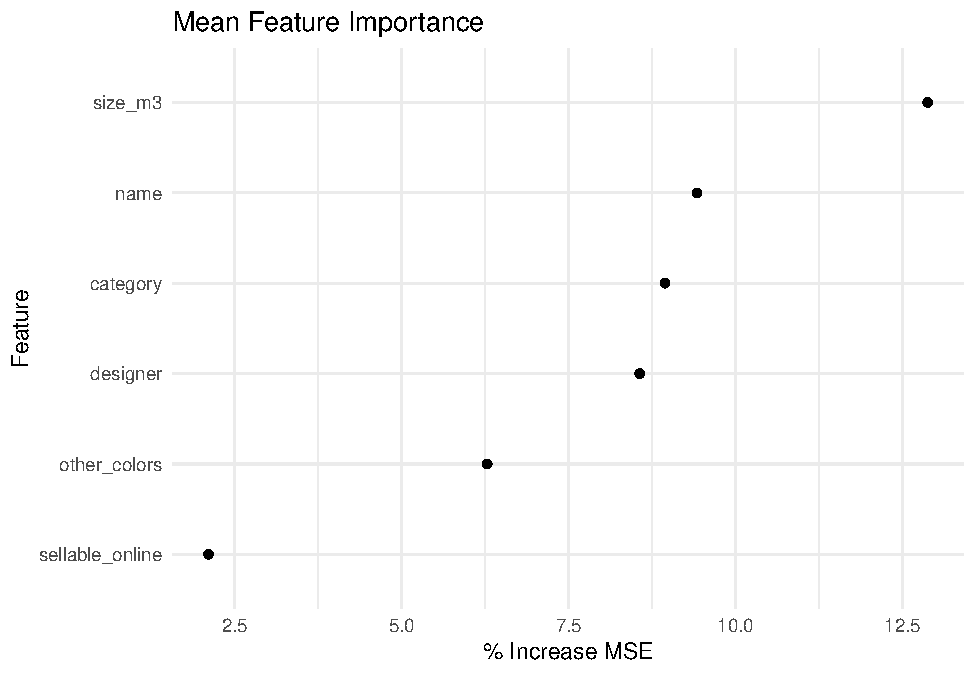
\includegraphics[width=0.9\linewidth]{_main_files/figure-latex/unnamed-chunk-4-1} \caption{A nice image.}\label{fig:unnamed-chunk-4}
\end{figure}

Thus, as can be seen in the figure above, the most important feature is \texttt{size\_m3} with an increase of the MSE of 182\%. The second, third and fourth most important features are \texttt{designer} with an increase of 120\%, \texttt{name} with an increase of 114\% and \texttt{category} with an increase of 105\%. The fifth most important feature is \texttt{other\_colors} with an increase of the MSE of 78\% and the least important feature is \texttt{sellable\_online} with a 9\% increase.

These results are further discussed in the following chapter.

\hypertarget{discussion}{%
\chapter{Discussion}\label{discussion}}

\hfill\textcolor{gray}{by J. Pein}

In this chapter, the results are discussed in connection with the research question. The question that the results were supposed to answer is the following:

\emph{How important are the different features of Ikea products in regard to their price?}

\hypertarget{feature-importance-1}{%
\section{Feature Importance}\label{feature-importance-1}}

The \texttt{size\_m3} variable is the most important feature. Probably the main reason for this is that the size of a product is closely linked to its material cost. Big items are generally more costly to produce, thus leading to a higher selling price and vice versa. Due to the high correlation to the price variable described in \ref{collinearity} and \ref{relationship}, it is worth discussing where or not to include this variable in a possible predictive analysis model.

The \texttt{designer} variable is the second most important feature. It might seem, that this is due to \emph{overfitting}, since the random forest regression model takes into account around 50 different combinations of designers, partly with a low number of occurences. But according to Grömping\footnote{``Variable Importance Assessment in Regression: Linear Regression versus Random Forest.''} random forest models are relatively robust against overfitting. Further research should be conducted to analyze whether overfitting is present or not.
When looking at the price distribution per designer, in can be clearly seen that the interquartile range (IQR) of price varies for each designer. In addition, the IQR often is smaller than 300€, thus showing a tendency towards a certain price range, which might be the reason for the relatively high feature importance of the designer variable. The plot @ref(price\_distribution\_designer) is available in the appendix.
The random forest regression model includes around 50 different product names with partly small numbers of occurences. Thus, the relatively high feature importance of the \texttt{name} variable might also be caused by overfitting. As discussed above, further research should be conducted to analyze whether this is the case.

\texttt{Category} is another feature with a relatively high importance. This is because the different category's price distributions show a clear tendency towards certain price segments @ref(price\_distribution\_category), i.e.~Wardrobes and beds are generally more expensive than chairs.
To the authors it seems counterintuitive that \texttt{designer} and \texttt{name} have higher feature importances than the \texttt{category} feature, because the IQR in the price distribution per category is often a lot smaller than the IQR of the designer and name price distributions. This also hints towards overfitting of the name and designer variables. However, in the categories with the most occurrences, namely \texttt{Wardrobes}, \texttt{Sofas\ \&\ armchairs} and \texttt{Beds}, the IQR is relatively large and there are many overlapping prices ranges for different categories, which explains a lower feature importance.

The feature importance of \texttt{other\_colors} is the second lowest, but still considerable. This still relatively high feature importance might be due to the difference of the mean price and the relatively small IQR @ref(price\_distribution\_other\_colors). On the other hand, there is a large overlapping area within the IQR in the two expressions of \texttt{other\_colors} possibly reducing the feature importance.

The very low feature importance of the \texttt{sellable\_online} variable is mainly because the low number of occurences of a product being sellable online. Only around 0.6\% of the products are sellable online.

\hypertarget{conclusion}{%
\section{Conclusion}\label{conclusion}}

Generally, the proposed random forest model was not validated with a test or validation data set. In further research, the results presented on the feature importance of different variables on the price variable should be validated by other techniques than used in this analysis to get unbiased results.

Also, the data was scraped from the arabian Ikea website online , thus this analysis mainly focusses on Ikea products in the Saudi Arabian market. To analyze the geographically independent feature importances, more data should be scraped from more international Ikea websites. The research question of this paper, \emph{How important are the different features of Ikea products in regard to their price?}, could thus not be answered for the global Ikea product market, but for the Saudi Arabian market only.

Furthermore, based on this analysis a predictive model could be developed which predicts the price of Ikea products in the Saudi Arabian Market based on the feature analyzed. This could be used by Ikea internally to analyze if the price of their new product aligns with the prices of the currently available product.

\hypertarget{individual-statements}{%
\chapter{Individual Statements}\label{individual-statements}}

\hypertarget{philip-kruxfcck}{%
\section{Philip Krück}\label{philip-kruxfcck}}

\hypertarget{johannes-pein}{%
\section{Johannes Pein}\label{johannes-pein}}

\startappendices

\hypertarget{appendix}{%
\chapter{Appendix}\label{appendix}}

\hypertarget{price_distribution_designer}{%
\section{Price Distribution per Designer}\label{price_distribution_designer}}

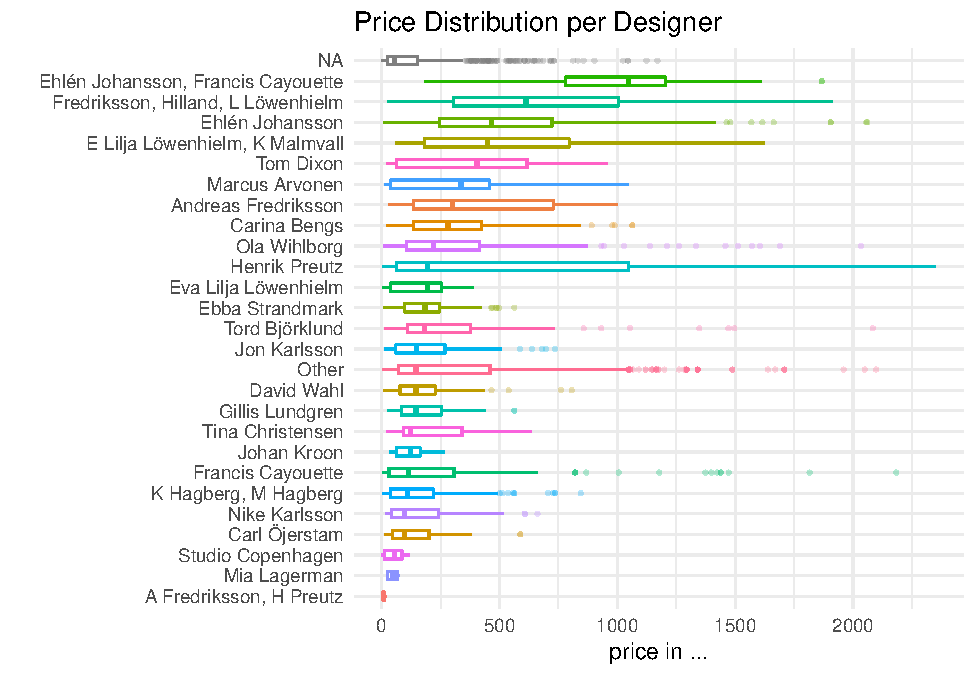
\includegraphics{_main_files/figure-latex/unnamed-chunk-5-1.pdf}

\hypertarget{price_distribution_category}{%
\section{Price Distribution per Category}\label{price_distribution_category}}

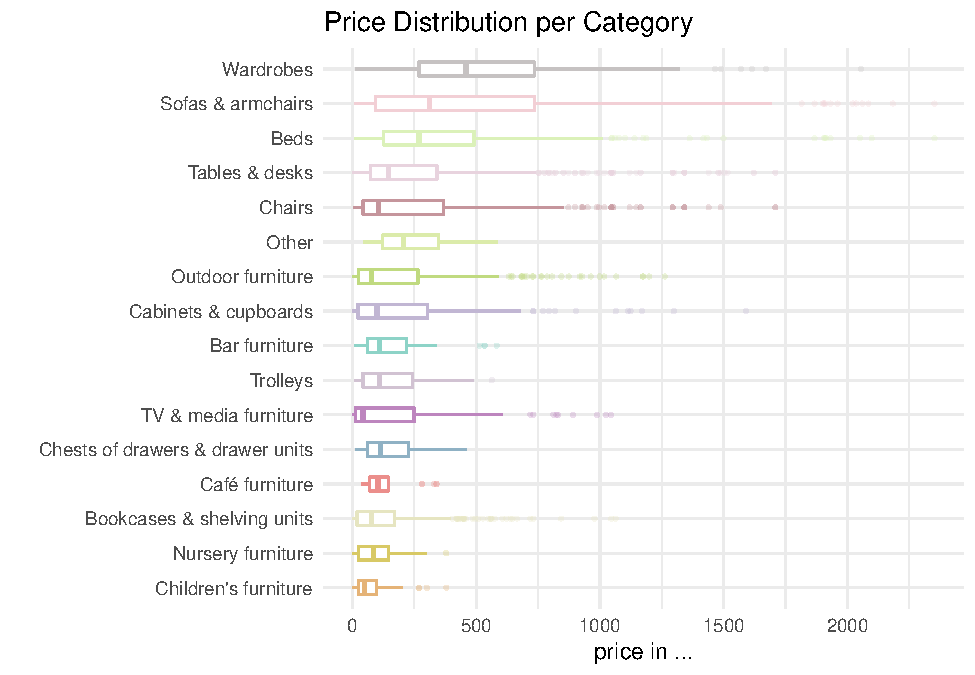
\includegraphics{_main_files/figure-latex/unnamed-chunk-6-1.pdf}

\hypertarget{price_distribution_other_colors}{%
\section{Price Distribution Other Colors}\label{price_distribution_other_colors}}

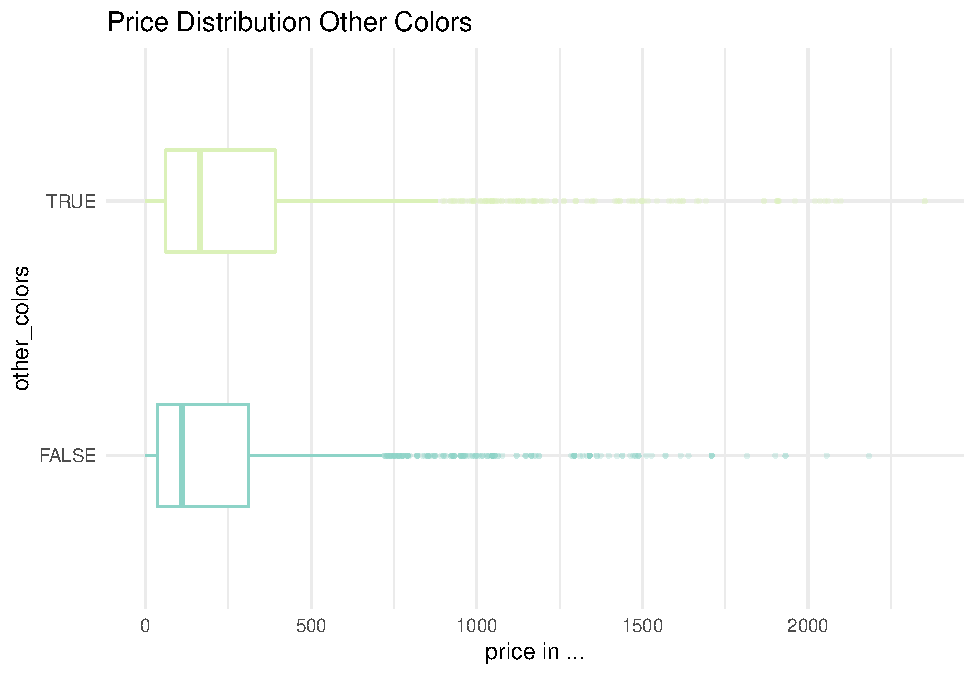
\includegraphics{_main_files/figure-latex/unnamed-chunk-7-1.pdf}

\hypertarget{price-distribution-sellable-online}{%
\section{Price Distribution Sellable Online}\label{price-distribution-sellable-online}}

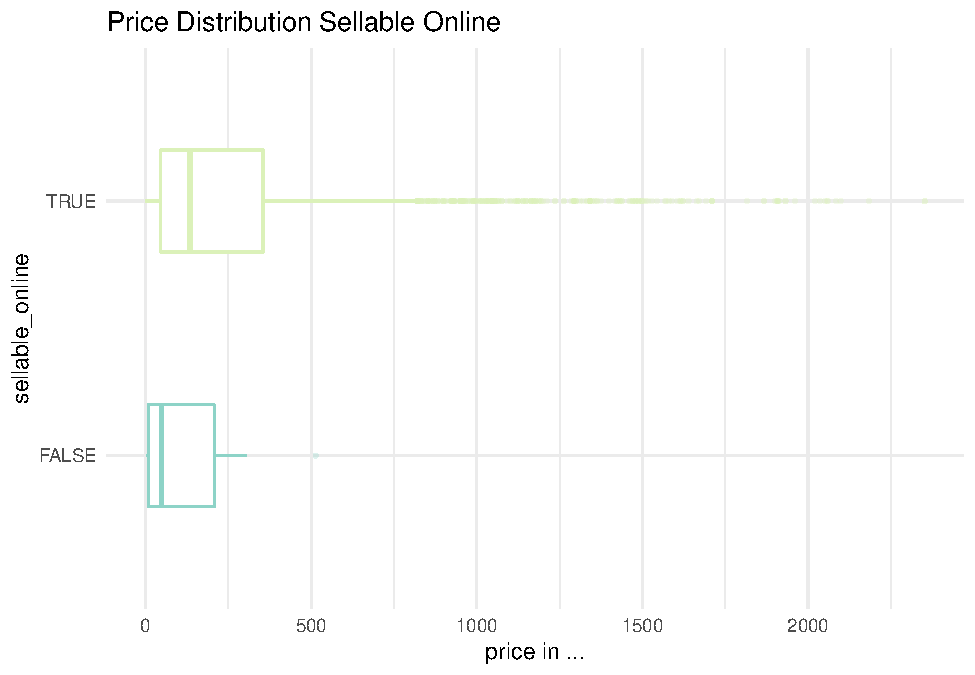
\includegraphics{_main_files/figure-latex/unnamed-chunk-8-1.pdf}

\hypertarget{relationship-between-independent-variables-and-price}{%
\section{Relationship between Independent Variables and Price}\label{relationship-between-independent-variables-and-price}}

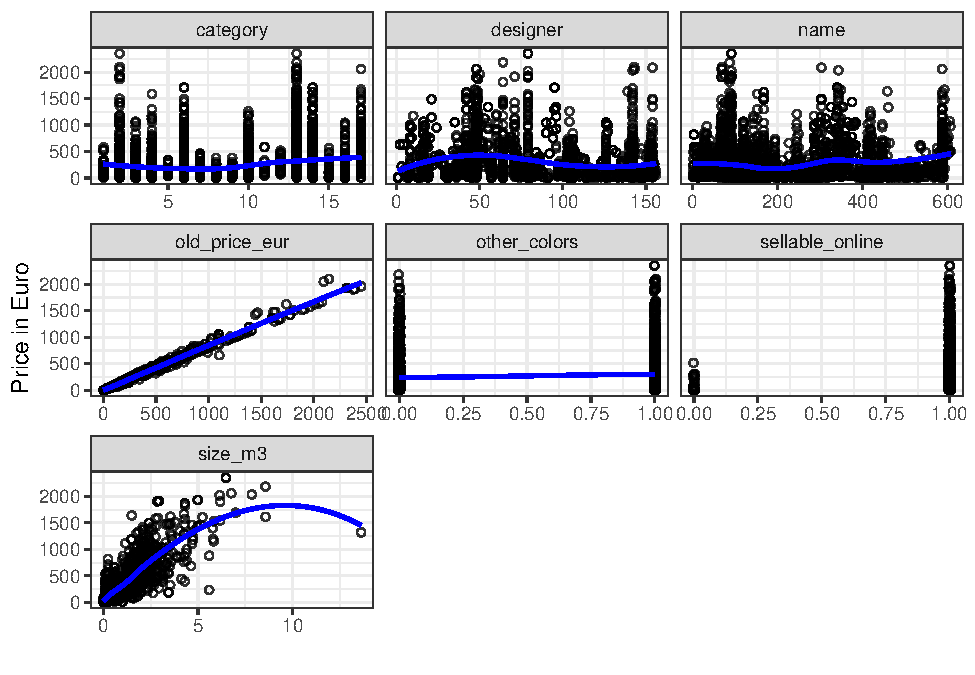
\includegraphics{_main_files/figure-latex/relationship-x-y-1.pdf}

\hypertarget{bibliography}{%
\chapter{Bibliography}\label{bibliography}}

\hypertarget{refs}{}
\leavevmode\hypertarget{ref-Groemping2009}{}%
Grömping, Ulrike. ``Variable Importance Assessment in Regression: Linear Regression versus Random Forest.'' \emph{The American Statistician}, nos. Vol. 63, No. 4 (2009): 308--19. \url{https://prof.beuth-hochschule.de/fileadmin/prof/groemp/downloads/tast_2E2009_2E08199.pdf}.

\leavevmode\hypertarget{ref-Liaw2002}{}%
Liaw, Andy, and Matthew Wiener. ``Classification and Regression by randomForest.'' \emph{R News}, nos. Vol. 2/3, December 2002 (2001). \url{https://www.researchgate.net/publication/228451484_Classification_and_Regression_by_RandomForest}.

\leavevmode\hypertarget{ref-Zuur2010}{}%
Zuur, E.N. Ieno lain. ``A protocol for data exploration to avoid common statistical problems.'' \emph{British Ecological Society}, 2010. doi:\href{https://doi.org/10.1145/1738826.1738829}{10.1145/1738826.1738829}.


%%%%% REFERENCES

% JEM: Quote for the top of references (just like a chapter quote if you're using them).  Comment to skip.
% \begin{savequote}[8cm]
% The first kind of intellectual and artistic personality belongs to the hedgehogs, the second to the foxes \dots
%   \qauthor{--- Sir Isaiah Berlin \cite{berlin_hedgehog_2013}}
% \end{savequote}

\setlength{\baselineskip}{0pt} % JEM: Single-space References

{\renewcommand*\MakeUppercase[1]{#1}%
\printbibliography[heading=bibintoc,title={\bibtitle}]}

\end{document}
